%
% General structure for the revdetua class:
%
\documentclass[...]{revdetua}
\usepackage{graphicx}

%
% Valid options are:
%
%   longpaper --------- \part and \tableofcontents defined
%   shortpaper -------- \part and \tableofcontents not defined (default)
%
%   english ----------- main language is English (default)
%   portugues --------- main language is Portuguese
%
%   draft ------------- draft version
%   final ------------- final version (default)
%
%   times ------------- use times (postscript) fonts for text
%
%   mirror ------------ prints a mirror image of the paper (with dvips)
%
%   visiblelabels ----- \SL, \SN, \SP, \EL, \EN, etc. defined
%   invisiblelabels --- \SL, \SN, \SP, \EL, \EN, etc. not defined (default)
%
% Note: the final version should use the times fonts
% Note: the really final version should also use the mirror option
%

\begin{document}

\Header{1}{25}{novembro}{2022}{0}
% Note: the month must be in Portuguese

\title{Finding the Minimum Weighted Closure of a Graph using Exhaustive Search and a Greedy Algorithm}
\author{Eduardo Santos, nºmec 93107, eduardosantoshf@ua.pt} % or \author{... \and ...}
\maketitle

\begin{abstract}
The objective of this assignment was to find a minimum weighted closure for a given vertex-weighted directed graph \textit{G(V, E)}, with \textit{n} vertices and \textit{m} edges. Exhaustive Search and Greedy Algorithms were used to solve this problem, with the solution explained in this paper, with both solutions being compared in terms of execution time, as well as complexity. The computations were made using a variety of parameters, which will also be referred on the following sections.
\end{abstract}

\section{Introduction}

A closure of \textit{G} is a set of vertices \textit{C}, such that no edges leave \textit{C}. The weight of a closure is the sum of its vertices’ weights. A \textbf{minimum weight closure} is a closure whose total weight is as small as possible. Both algorithms used computed the minimum weighted closure of a given graph, with each approach and its parameters explained later on.

\section{ Problem Description}

To solve this problem, the first thing to do was to create a random graph, so that it could be used to compute the minimum weighted closure. To do this, the NetworkX\cite{networkx} library was used, which is a potent tool for creating, manipulating, and studying the structure, dynamics, and functions of complex networks, or graphs.
To better understand this problem, let's consider a graph with 5 nodes and 5 edges, represented in the figure below. In this particular case, and in order to facilitate the explanation, a graph with multiple closures was used. Let's also consider each node's number as its weight. 

\begin{figure}[!htb]
    \centering
    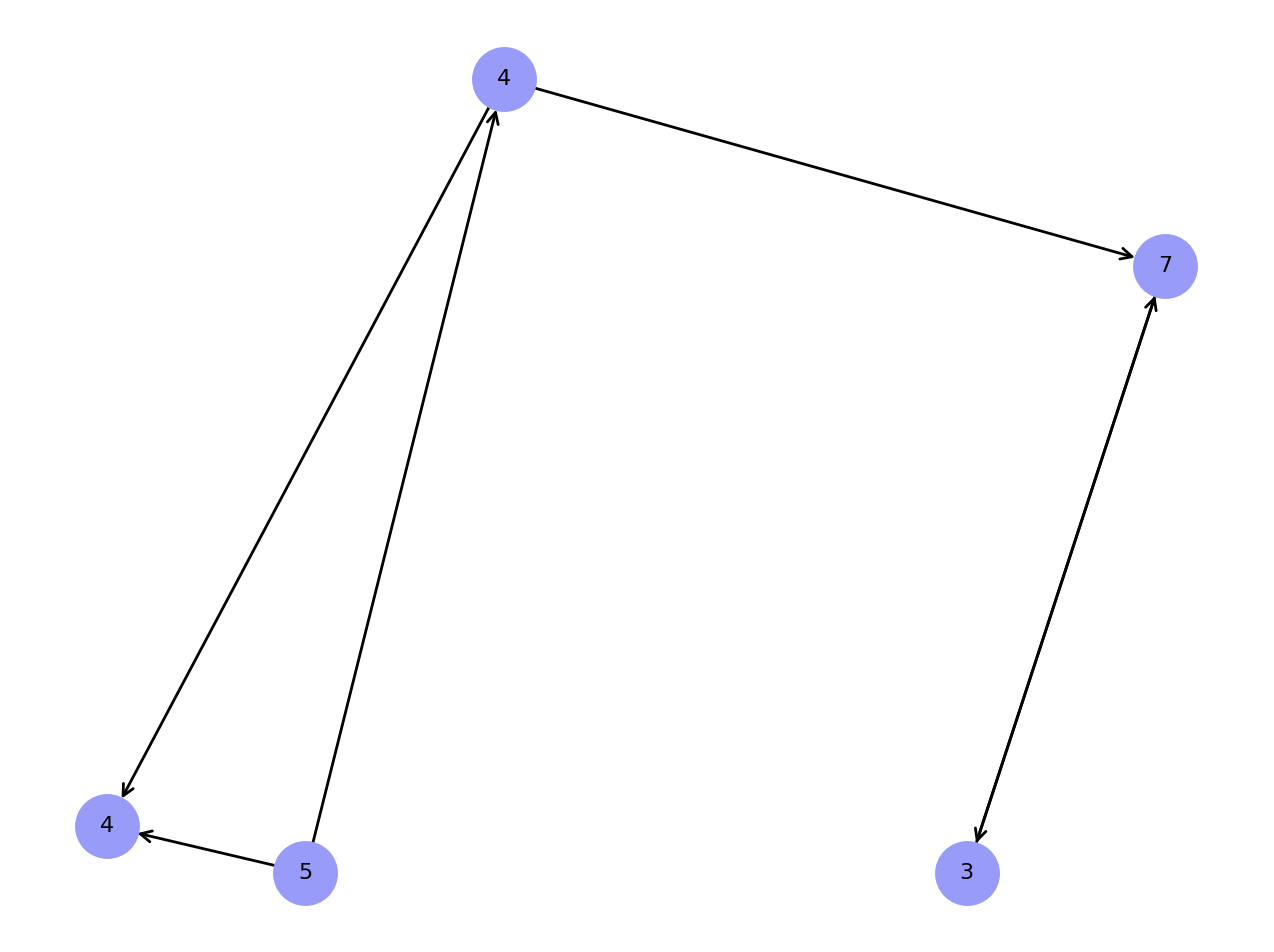
\includegraphics[width=0.75\columnwidth]{./figures/simple_graph.png}
    \caption{Example of a Simple Graph}
    \label{fig:Simple Graph}
\end{figure}

The graph above has 5 sets that are closures:

\begin{itemize}
    \item 4 (weight: 4)
    \item 3, 7 (weight: 10)
    \item 3, 7, 4 (weight: 14)
    \item 3, 7, 4, 4 (weight: 18)
    \item 3, 7, 4, 4, 5 (whole graph) (weight: 23)
\end{itemize}

Therefore, the minimum weighted closure of this graph is 4, as it represents the minimum sum of closure vertices' weights.

\section{ Implementation Description}

Running the main program, there are a few flags that can be used, depending on what we wish to compute, etc.

\begin{figure}[!htb]
    \centering
    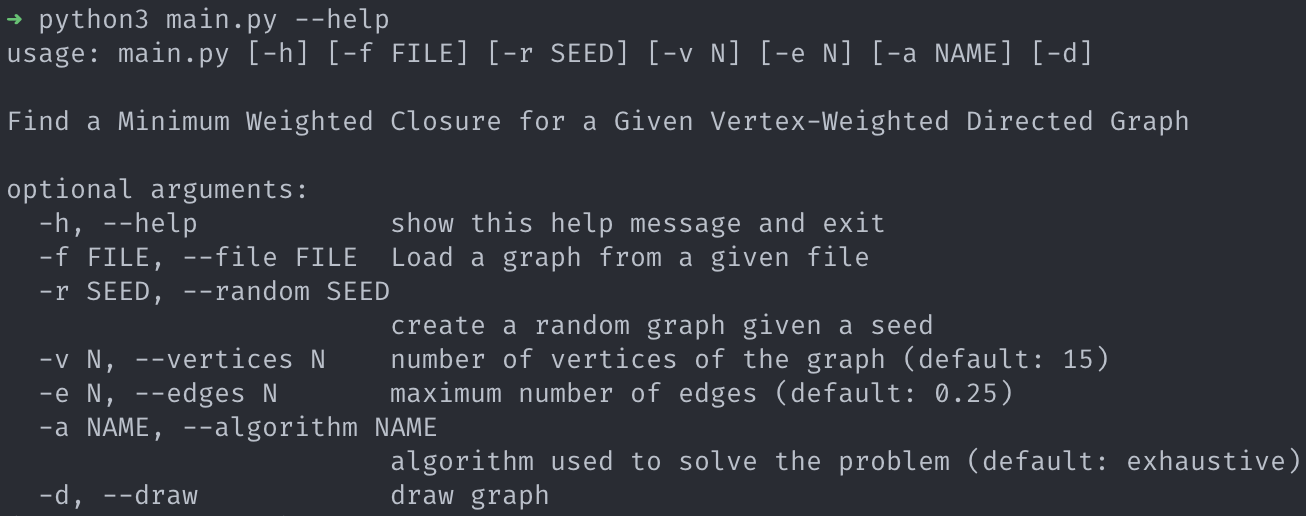
\includegraphics[width=1\columnwidth]{./figures/program_help}
    \caption{Help Menu of the Main Program}
    \label{fig:Help Menu}
\end{figure}

To compute using both the exhaustive and the greedy search, there are two options to create a graph. Using the \textbf{-f} flag, a graph can be read from a file, with the following format:
\begin{verbatim}
4
1 1 9
1 2 5 3
2 3 4 1 2
3 5 7 2
\end{verbatim}

The first line represents the number of nodes in the graph, and each following line represents the \textbf{\textit{x} coordinate}, \textbf{\textit{y} coordinate}, \textbf{node weight}, and the \textbf{node(s) to which it connects}, all separated by spaces.

Using the \textbf{-r} flag, the program generates a random graph, using a student number as a seed, and the number of nodes given by the \textbf{-n} flag. Each node's coordinates are randomly generated values from 1 to 20, and it only adds a node if the point did not already exist. Also, when generating random edges, the flag \textbf{-e} is used to set the maximum number of edges of the graph to be generated. For the computations, which will be discussed later in this paper, the values 12.5\%, 25\%, 50\%, and 75\% will be used as the maximum number of edges.

The \textbf{graph.py} contains the \textbf{Graph}, \textbf{GraphDrawer}, \textbf{ExhaustiveSearch}, and the \textbf{GreedySearch} classes. In the \textbf{Graph} class, there are two methods to help with the definition of a graph:

\begin{itemize}
    \item \textit{add\_node(self, node: Point, weight: int)} - this method saves the nodes in a dictionary, with the node coordinates as key, and the node's weight as value.
    \item \textit{add\_edge(self, node1: Point, node2: Point)} - this method saves the edges also on a dictionary, with \textit{node1} as key, and adding the \textit{node2} to the first one's key list. This is helpful when the problem uses a directed graph, because of the starting/ending node of an edge matter, regarding its order.
\end{itemize}

There is also the flag \textbf{-a} to choose between the exhaustive and the greedy algorithms, with the first one being the default one, and the \textbf{-d} flag, which allows drawing the graph, using the Matplotlib\cite{matplotib} library.

In the graph below, the minimum weighted closure is presented with the color green. This solution was computed using the exhaustive algorithm.

\begin{figure}[!htb]
    \centering
    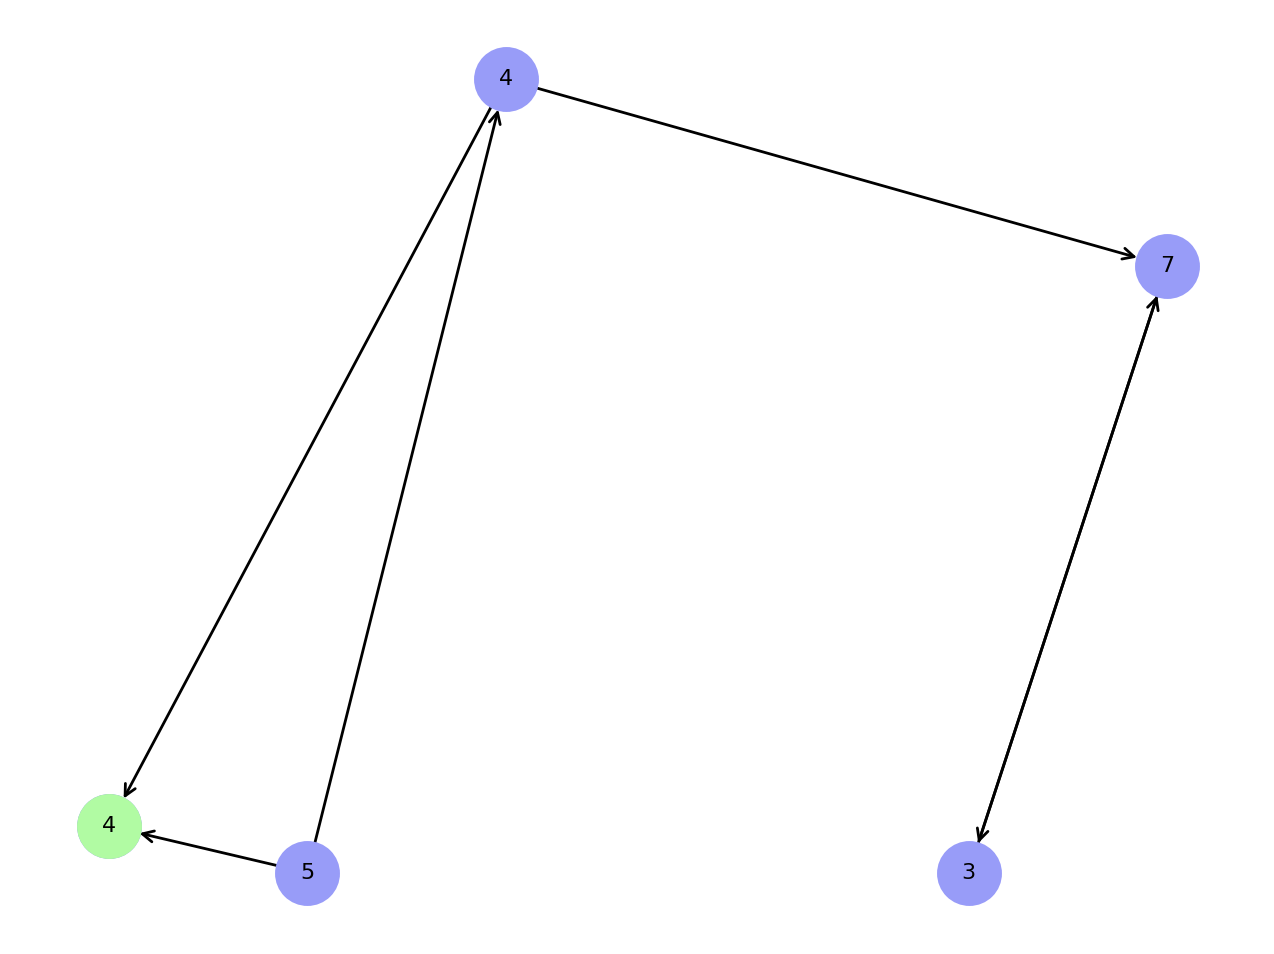
\includegraphics[width=0.75\columnwidth]{./figures/simple_graph_exhaustive_solution.png}
    \caption{Minimum Weighted Closure Using the Exhaustive Algorithm}
    \label{fig:Minimum Weighted Closure Using the Exhaustive Algorithm}
\end{figure}

On the contrary, using the greedy algorithm, a different solution was found. This solution's minimum weighted closure is also represented with the color green, in the graph below.

\begin{figure}[!htb]
    \centering
    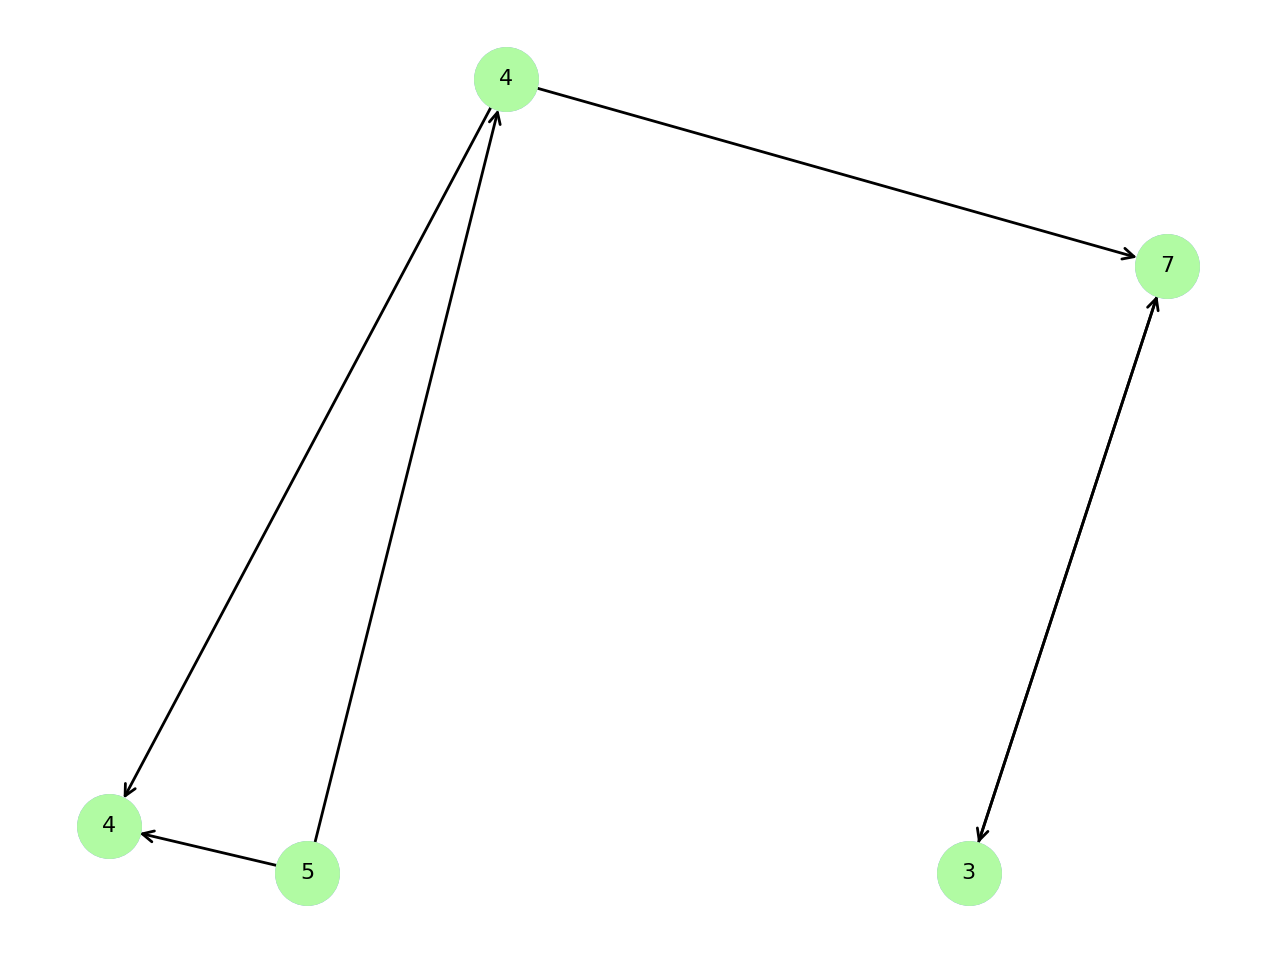
\includegraphics[width=0.75\columnwidth]{./figures/simple_graph_greedy_solution.png}
    \caption{Minimum Weighted Closure Using the Greedy Algorithm}
    \label{fig:Minimum Weighted Closure Using the Greedy Algorithm}
\end{figure}

In this specific case, the whole graph is considered by the algorithm as the minimum weighted closure. The reason for that will be later on explained.

\subsection{Exhaustive Search}

Regarding the exhaustive search, firstly the power set of the set of nodes is computed. The power set of a set S is the set of all subsets of S, including the empty set and S itself, of size 1 to N, where N is the total number of nodes. In this case, every subset is considered a possible closure. Then, for every subset, \textit{C}, it is necessary to check if there are any edges for other nodes that are not in \textit{C}. If this happens, then \textit{C} is not a closure, if not, then the subset is added to the \textit{closures} list. After having all closures, every subset node's weight is added, and the closure with the smallest sum is considered the minimum weighted closure.

\subsubsection{Formal Computational Complexity Analysis}


\subsection{Greedy Search}

Regarding the greedy search, 

\subsubsection{Formal Computational Complexity Analysis}



\section{Results and Discussion}


\begin{table}[!htb]
\resizebox{0.45 \textwidth}{!}{%
\begin{tabular}{||c c c c c||}
 \hline
 V & E & Operations  & Tested Sols. & Exec.Time(ms) \\ [0.2ex] 
 \hline\hline
 5 & 5 & 52 & 31 & 0.04 \\ 
 \hline
 7 & 13 & 166 & 127 & 0.19 \\
 \hline
 10 & 21 & 1234 & 1023 & 0.98\\
 \hline
 15 & 45 & 42924 & 32767 & 32.84 \\
 \hline
 17 & 41 & 141971 & 131071 & 108.18 \\
 \hline
 20 & 55 & 1624913 & 1048575 & 1250.05 \\
 \hline 
 25 & 131 & 33686474 & 33554431 & 33705.21 \\
 \hline 
 30 & 167 & 1576111704 & 1073741823 & 1910669.58 \\ [1ex] 
 \hline
\end{tabular}
%
}
\caption{\label{tab:table-name}Obtained results for the Exhaustive Approach}
\end{table}
 

\begin{table}[!htb]
\resizebox{0.45 \textwidth}{!}{%
\begin{tabular}{||c c c c c||}
 \hline
 V & E & Operations  & Tested Sols. & Exec.Time(ms) \\ [0.2ex] 
 \hline\hline
 5 & 5 & 12 & 5 & 0.017 \\ 
 \hline
 7 & 13 & 18 & 7 & 0.019 \\
 \hline
 10 & 21 & 19 & 10 & 0.020 \\
 \hline
 15 & 45 & 42924 & 15 & 0.025 \\
 \hline
 17 & 41 & 44 & 17 &  0.035 \\
 \hline
 20 & 55 & 48 & 20 & 0.038 \\
 \hline 
 25 & 131 & 55 & 25 & 0.05 \\
 \hline 
 30 & 167 & 85 & 30 &  0.067 \\ 
 \hline 
... & ... & ... & ... & ... \\
 \hline 
 100 & 1772 & 199 & 100 &  0.303 \\[1ex] 
 \hline
\end{tabular}
%
}
\caption{\label{tab:table-name}Obtained results for the Greedy Approach}
\end{table}
 



\section{Conclusion}


\begin{thebibliography}{9}

\bibitem{networkx}
NetworkX developers. (2014-2022). NetworkX. 
\url{https://networkx.org/}

\bibitem{matplotib}
The Matplotlib development team. (2012-2022). Matplotlib. \url{https://matplotlib.org/}
\end{thebibliography}




% use a field named url or \url{} for URLs
% Note: the \bibliographystyle is set automatically

\end{document}
